\documentclass{standalone}
\usepackage{xcolor}
\usepackage{forest}
\usepackage{tikz}
\begin{document}
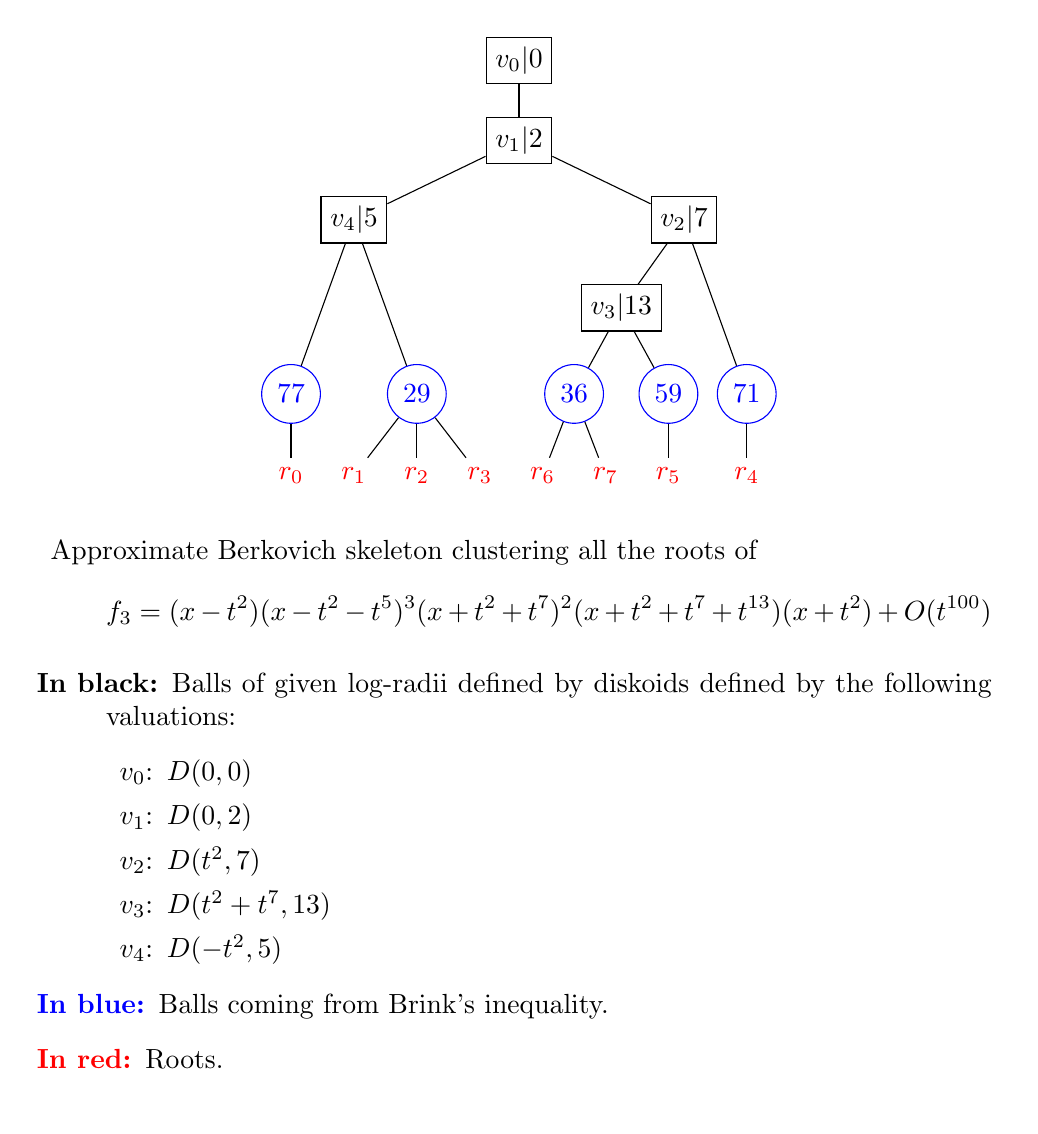
\begin{tikzpicture}
\node[anchor=north] (tree) at (0,0) {
\begin{forest}
[$v_{0} \vert 0$, draw,  black[$v_{1} \vert 2$, draw,  black[$v_{4} \vert 5$, draw,  black[$77$, circle, draw,  blue, tier=Brink[$r_{0}$,  red, tier=root]
]
[$29$, circle, draw,  blue, tier=Brink[$r_{1}$,  red, tier=root]
[$r_{2}$,  red, tier=root]
[$r_{3}$,  red, tier=root]
]
]
[$v_{2} \vert 7$, draw,  black[$v_{3} \vert 13$, draw,  black[$36$, circle, draw,  blue, tier=Brink[$r_{6}$,  red, tier=root]
[$r_{7}$,  red, tier=root]
]
[$59$, circle, draw,  blue, tier=Brink[$r_{5}$,  red, tier=root]
]
]
[$71$, circle, draw,  blue, tier=Brink[$r_{4}$,  red, tier=root]
]
]
]
]
\end{forest}
};
\node[anchor=north, align=center] at (tree.south) {
    \parbox{\linewidth}{%
        \centering
        \begin{description}
                	\item[] Approximate Berkovich skeleton clustering all the roots of   \[f_3=(x-t^2)(x-t^2-t^5)^3(x+t^2+t^7)^2(x+t^2+t^7+t^{13})(x+t^2)+O(t^{100})\]
            \item[In black:] Balls of given log-radii defined by diskoids defined by the following valuations:  
                \begin{itemize}
                    \item[ $v_{ 0 }$:] $D(0,0)$
                    \item[ $v_{ 1 }$:] $D(0,2)$
                    \item[ $v_{ 2 }$:] $D(t^2,7)$
                    \item[ $v_{ 3 }$:] $D(t^2+t^7,13)$
                    \item[ $v_{ 4 }$:] $D(-t^2,5)$
                \end{itemize}
            \item[\textcolor{blue}{ In blue:}] Balls coming from Brink's inequality.
            \item[\textcolor{red}{In red:}] Roots.
        \end{description}%
    }
};
\end{tikzpicture}
\end{document}